\chapter{Ten Minutes in the Image}
\label{ch:tenminutes}

\standfirst{The interface is from 1983 and it has two habits that make a
working system look broken. Learn them now and the rest is easy.}

\section{Two habits}

\subsection{Menus are press-and-hold}

There is no click-to-open menu anywhere in this interface. \textbf{Press the
button and keep it down.} The menu stays up only while you hold it. Drag onto
the item you want and release there.

A click---press and release in the same instant---puts the menu up and takes
it straight back down, and looks exactly like nothing happened.

\subsection{You place a window yourself}

Choosing \ct{browser} from a menu does not open a window. It \emph{arms} one.
The next thing the system wants is for you to say where it goes: press the
left button, drag out a rectangle, release. The window appears when you let go.

Nothing tells you this in words. The only signal is the cursor, which turns
into a top-left corner, then a bottom-right corner while you drag, then back
to an arrow when the window appears.

\begin{stwarn}[The single most common way to conclude this is broken]
Choose \ct{browser} and then wait. Nothing happens, forever, and it looks
exactly like a hang. The system is not slow---measured end to end, opening a
System Browser takes 1.1 seconds. It is waiting for you.
\end{stwarn}

\section{The three buttons}
\label{sec:buttons}

Smalltalk-80 names mouse buttons by colour, after the Alto's, and the library
still does. On an ordinary three-button mouse:

\begin{center}
\small
\begin{tabular}{@{}llp{0.52\textwidth}@{}}
\toprule
button & 1983 called it & what it does\\
\midrule
left   & red    & select: text, list items, everything\\
middle & yellow & the \emph{view's} own menu---what you can do to the contents\\
right  & blue   & the \emph{window's} menu---move it, close it\\
\bottomrule
\end{tabular}
\end{center}

If you have a two-button mouse or a trackpad, you will need whatever your
system offers for a middle click, because the middle button is the one you
use most.

The middle column is there because the library still speaks in colours: the
Alto's buttons were painted red, yellow and blue, and the source you will
read says \ct{yellowButtonMenu} and \ct{redButtonPressed} throughout. This
book says left, middle and right everywhere else.

\section{Opening your first window}

Start the desktop:

\begin{sh}
./st80 -run st80.image
\end{sh}

You get a grey halftone desktop with nothing on it. Now:

\begin{enumerate}
\item Press and \emph{hold} the \textbf{middle} button anywhere on
  the desktop. The system menu appears:
\begin{plain}
restore display
exit project
------------------
project
file list
browser
workspace
system transcript
system workspace
------------------
save
quit
\end{plain}
\item Still holding, drag down to \ct{workspace} and release.
\item The cursor becomes a corner. Press the \textbf{left} button
  somewhere in the upper left, drag down and right to sketch a rectangle, and
  release.
\end{enumerate}

A window appears with a label tab reading \ct{Workspace}. A workspace is a
scratch pad: text you can type in and evaluate, saved nowhere.

\begin{figure}[htbp]
\centering
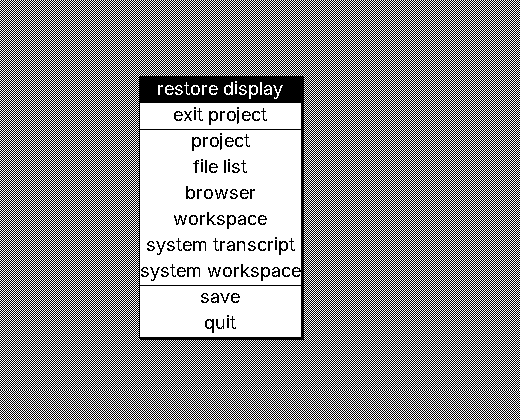
\includegraphics[width=0.78\textwidth]{figures/desktop-menu.png}
\caption{The desktop menu, held open with the middle button. The grey
halftone behind it is the bare desktop. \ct{restore display} is highlighted
because the pointer was warped onto the menu's current item when it
opened---that jump is deliberate, and Section~3.7 says why.}
\end{figure}

\section{Evaluating something}

Click in the workspace and type:

\begin{st}
3 + 4
\end{st}

Now select it---press the left button at the start, drag to the end,
release---and with the text still selected press and hold the \textbf{middle}
button. This menu
is the text editor's:

\begin{plain}
again
undo
-----------
copy
cut
paste
-----------
do it
print it
-----------
accept
cancel
\end{plain}

Drag to \ct{print it} and release. The answer is inserted after your selection
and left selected, so you can type over it:

\begin{st}
3 + 4 7
\end{st}

\ct{do it} evaluates and discards the answer; \ct{print it} evaluates and
shows it. Those two are the whole of how you talk to a running Smalltalk.

\begin{stnote}[There are no keyboard shortcuts for this]
If you have used Pharo or Squeak you will reach for \ct{Ctrl-D} and
\ct{Ctrl-P}. They are not here. In 1983 \ct{do it} and \ct{print it} live in
the middle-button menu and nowhere else, and this system is that system.
\end{stnote}

Try a few more. Select each line and \ct{print it}:

\begin{st}
100 factorial

(1 to: 10) inject: 0 into: [:a :b | a + b]

Smalltalk classNames size

#(3 1 2) asSortedCollection asArray
\end{st}

\section{Moving and closing a window}

There is no title bar to drag and no close box. Hold the \textbf{right}
button anywhere over a window:

\begin{plain}
under
move
frame
collapse
----------
close
\end{plain}

\begin{description}
\item[under] send this window behind the ones it overlaps
\item[move] pick the window up
\item[frame] ask for a new rectangle, the way opening did
\item[collapse] shrink it to just its label tab, which still has this menu
\item[close] close it
\end{description}

\ct{move} has a second step that surprises everybody. When you release on
\ct{move}, \textbf{the window follows the pointer with no button held down},
and you \emph{click} to drop it. That is not a slip: the 1983 code tracks
\emph{while no button is pressed}, which is the opposite of every drag written
since.

\section{The pointer jumps onto the menu}

When a menu opens, the cursor is warped onto its current item. That is
deliberate---it is the second line of \ct{PopUpMenu>>startUp:}---and it is
what makes a menu near the edge of the screen usable, because the menu moves
to stay on screen and the pointer follows it.

\section{Opening a Browser}

Same gesture: middle button on the desktop, drag to \ct{browser}, release,
then frame
a rectangle---make this one large, most of the screen.

\begin{figure}[htbp]
\centering
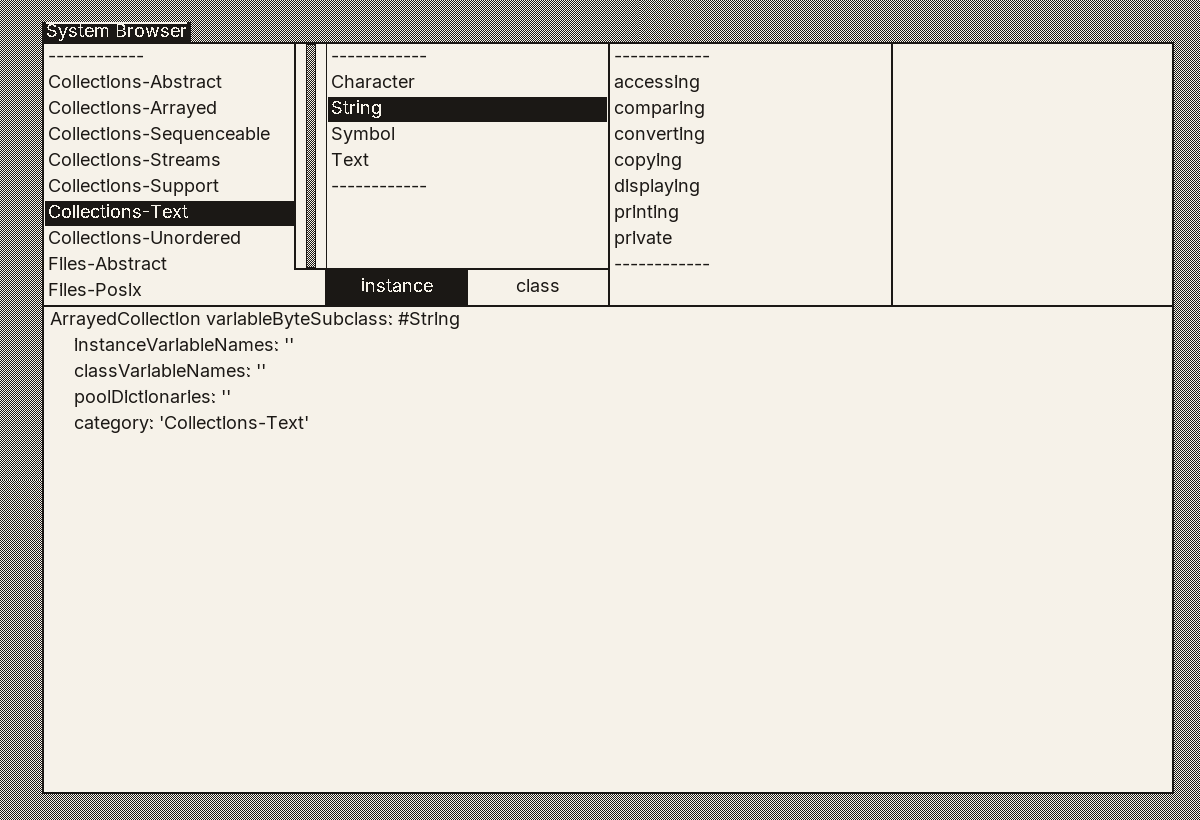
\includegraphics[width=\textwidth]{../doc/desktop.png}
\caption{The System Browser. Four panes across the top---categories, classes,
message categories, messages---and the code for whatever is selected below.
The \ct{instance} and \ct{class} buttons under the class list switch which
side you are looking at.}
\end{figure}

Click along the top panes with the left button: pick a category on the left,
then a class, then a message category, then a message. The bottom pane fills
with the source of the method you chose. It is editable, and \ct{accept} in
the middle-button menu compiles it back into the running system.

That is the whole idea of Smalltalk, and it is worth pausing on. The Browser
you are using is written in the language you are browsing, its source is in
the list you are reading, and if you change it the change takes effect in the
window you changed it from.

\section{Leaving}

Middle button on the desktop, then \ct{quit}, which offers three choices:
save and
quit, quit without saving, or continue. Closing the operating-system window
also works and saves nothing.

\begin{stwarn}
Nothing is saved automatically. Everything you typed and every method you
accepted lives only in memory until you save the image.
Chapter~\ref{ch:keeping} is about how to keep work, and it is worth reading
before you have anything you would mind losing.
\end{stwarn}

\section{If the mouse does nothing}

Then the display was resized without the image being told, and no controller
believes the cursor is inside it. Run with \ctp{ST\_DISPLAY\_TRACE=1} and the
system will name the step that refused. This is a known failure mode with a
known cause; see Appendix~\ref{app:trouble}.
